\section{Performance Evaluation}
\subsection{Experimental Setup}

\noindent
\textbf{Datasets, Backbones, and Baselines:} We evaluate on CIFAR-100~\cite{krizhevsky2009learning} (DeiT-Tiny~\cite{touvron2021training}), CASIA-Iris~\cite{singh2017gender} (LAM~\cite{luo2025novel}), Sokoto Coventry fingerprints~\cite{shehu2018sokoto} (JIPNet~\cite{guan2024joint}), and CASIA-Face100~\cite{yi2014learning} (Face Transformer~\cite{zhong2021face}), comparing CU against SCRUB~\cite{kurmanji2023towards}, SalUn~\cite{fan2023salun}, GS-LoRA~\cite{zhao2024continual}, LTU~\cite{huang2024learning}, MCU~\cite{shi2025mcu}, and Forget Vectors~\cite{sun2024forget}, plus an Oracle trained only on $D_r^{\textbf{full}}$ as the upper bound.

\vspace{0.2cm}
\noindent
\textbf{Evaluation Metrics:} We report $Acc_f$, $Acc_r$, MIA (label-only attack~\cite{choquette2021label}, $\approx 0.5$ = safe), KL divergence to Oracle, RTE, and H-Mean~\cite{shibata2021learning}. Success requires $Acc_f \approx 0$, $Acc_r \approx$ Oracle, low KL/RTE. FAR@$\{0.3,0.4,0.5\}$/EER (cosine similarity, forget probes vs.\ retain gallery) further verify open-set identity confusion (Section~\ref{sec:attack}).

\subsection{Main Results}
\label{sec:main-results}
Table~\ref{tab:all} presents results across four tasks: classification, iris recognition, fingerprint recognition, and face recognition, where \colorbox{green!30}{green} highlights best performance and \colorbox{blue!30}{blue} indicates second-best.

\begin{table*}[!ht]
\centering
\small
\renewcommand{\arraystretch}{1.0}
\resizebox{\textwidth}{!}{%
\begin{tabular}{l|w{c}{1.1cm}w{c}{1.1cm}w{c}{1.1cm}w{c}{1.1cm}w{c}{1.1cm}w{c}{1.1cm}|w{c}{1.1cm}w{c}{1.1cm}w{c}{1.1cm}w{c}{1.1cm}w{c}{1.1cm}w{c}{1.1cm}}
\toprule
\multirow{2}{*}{\textbf{Method}}
& \multicolumn{6}{c|}{\textbf{Classification}} & \multicolumn{6}{c}{\textbf{Iris recognition}} \\
\cmidrule(lr){2-7} \cmidrule(lr){8-13}
& $Acc_f{\downarrow}$ & $Acc_r{\uparrow}$ & $H\text{-}Mean{\uparrow}$ & KL${\downarrow}$ & MIA$\downarrow$ & RTE${\downarrow}$
& $Acc_f{\downarrow}$ & $Acc_r{\uparrow}$ & $H\text{-}Mean{\uparrow}$ & KL${\downarrow}$ & MIA$\downarrow$ & RTE${\downarrow}$ \\
\midrule
Oracle        & --   & 77.36 & --    & --   & --   & --     & --   & 99.03 & --   & --   & --   & --    \\
\midrule
GS-LoRA~\cite{zhao2024continual}    & 0.11 & 71.32 & 74.18 & \colorbox{green!30}{0.73} & \colorbox{blue!30}{0.56} & \colorbox{blue!30}{153.2} & 0.00 & 93.42 & 96.18   & \colorbox{green!30}{0.75} & 0.69 & \colorbox{blue!30}{225.7} \\
SalUn~\cite{fan2023salun}           & 0.37 & 72.46 & 74.63 & 1.32 & 0.63 & 225.6 & 0.37 & 92.37 & 95.44 & \colorbox{blue!30}{0.79} & 0.59 & 427.2 \\
SCRUB~\cite{kurmanji2023towards}    & 0.58 & 73.11 & 74.90 & 1.89 & 0.64 & 219.3 & 0.43 & 95.58 & 97.07 & 0.83 & 0.63 & 501.8 \\
FV~\cite{sun2024forget}             & 0.00 & 74.43 & \colorbox{blue!30}{75.89} & 0.87 & \colorbox{green!30}{0.55} & 189.5 & 0.00 & 96.27 & 97.63   & 1.13 & 0.57 & 383.1 \\
MCU~\cite{shi2025mcu}               & 0.42 & 74.43 & 75.66 & 0.87 & 0.59 & {175.5} & 0.00 & \colorbox{green!30}{98.87} & \colorbox{green!30}{98.95}   & 0.99 & 0.63 & 437.2 \\
LTU~\cite{huang2024learning}        & 0.00 & \colorbox{green!30}{76.32} & \colorbox{green!30}{76.83} & \colorbox{green!30}{0.75} & 0.57 & 239.3 & 0.73 & 95.43 & 96.85 & 1.25 & \colorbox{blue!30}{0.55} & {329.4} \\
\midrule
\rowcolor{pink!15}
\textbf{CU}   & 0.47 & \colorbox{blue!30}{74.46} & 75.65 & {1.27} & \colorbox{blue!30}{0.56} & \colorbox{green!30}{55.5}  & 0.06 & \colorbox{blue!30}{97.89} & \colorbox{blue!30}{98.43} & 1.01 & \colorbox{green!30}{0.53} & \colorbox{green!30}{116.1} \\
\midrule
\addlinespace[0.15cm]
\midrule
\multirow{2}{*}{\textbf{Method}}
& \multicolumn{6}{c|}{\textbf{Fingerprint recognition}} & \multicolumn{6}{c}{\textbf{Face recognition}} \\
\cmidrule(lr){2-7} \cmidrule(lr){8-13}
& $Acc_f{\downarrow}$ & $Acc_r{\uparrow}$ & $H\text{-}Mean{\uparrow}$ & KL${\downarrow}$ & MIA$\downarrow$ & RTE${\downarrow}$
& $Acc_f{\downarrow}$ & $Acc_r{\uparrow}$ & $H\text{-}Mean{\uparrow}$ & KL${\downarrow}$ & MIA$\downarrow$ & RTE${\downarrow}$ \\
\midrule
Oracle        & --   & 90.82 & --    & -- & --   & --   & --   & 95.12   & --   & --   & --   & --   \\
\midrule
GS-LoRA~\cite{zhao2024continual}    & 0.00   & 83.42   & 86.98    & 1.13    & 0.65   & \colorbox{blue!30}{155.3}   & 0.57   & 93.25   & \colorbox{blue!30}{93.90}  & 1.13   & \colorbox{blue!30}{0.53}   & \colorbox{blue!30}{284.4}   \\
SalUn~\cite{fan2023salun}           & 0.10   & 82.32   & 86.24    & \colorbox{green!30}{0.75}    & 0.63   & 202.2   & 0.00   & 90.15   & 92.56  & 1.27   & 0.59   & 417.2   \\
SCRUB~\cite{kurmanji2023towards}    & 0.00   & 83.27   & 86.85    & 2.36    & 0.57   & 175.3   & 0.42   & \colorbox{blue!30}{93.27}   & 93.98  & 2.87   & 0.63   & 389.5   \\
FV~\cite{sun2024forget}             & 0.30   & 84.44   & 87.38    & 1.27    & \colorbox{green!30}{0.54}   & 160.7   & 0.20   & 92.27   & 93.58  & 1.20   & 0.60   & {380.3}   \\
MCU~\cite{shi2025mcu}               & 0.00   & 80.32   & 85.24    & \colorbox{blue!30}{0.99}    & 0.59   & 220.5   & 0.00   & 90.12   & 92.54  & \colorbox{green!30}{0.89}   & 0.57   & 403.8   \\
LTU~\cite{huang2024learning}        & 0.00   & \colorbox{green!30}{ 87.72}   & \colorbox{green!30}{89.24}    & 1.13    & \colorbox{green!30}{0.54}   & 237.4   & 0.00   & 92.58   & 93.84  & \colorbox{blue!30}{0.93}   & 0.55   & 430.2   \\
\midrule
\rowcolor{pink!15}
\textbf{CU}   & 0.00   & \colorbox{blue!30}{87.23}   & \colorbox{blue!30}{88.98}    & {1.05}    & \colorbox{blue!30}{0.55}   & \colorbox{green!30}{55.32}   & 0.00   & \colorbox{green!30}{93.98}   & \colorbox{green!30}{94.55}   & {1.67}   & \colorbox{green!30}{0.51}   & \colorbox{green!30}{175.3}   \\
\bottomrule
\end{tabular}%
}
\caption{Comprehensive performance evaluation across four recognition domains. Proposed CU achieves 3--4$\times$ speedup in runtime efficiency (RTE) while maintaining competitive forgetting, retention, and privacy metrics
.}
\label{tab:all}
\end{table*}

\vspace{0.2cm}
\noindent
\textbf{Unlearning and Retention:} All methods achieve near perfect forgetting $Acc_f < 1\%$, approaching random assignment. Proposed CU consistently ranks first or second in $Acc_r$ across all tasks, with LTU as the strongest competitor on classification, iris, and fingerprint tasks, while MCU excels on iris recognition. For \textit{H-Mean}, proposed CU alternates between first and second positions alongside competitive showings from LTU, FV, MCU, and GS-LoRA.

\vspace{0.2cm}
\noindent
\textbf{Privacy and Efficiency:} GS-LoRA achieves lower KL divergence than CU, which is expected since CU deliberately modifies logit distributions to suppress forget classes and is therefore less competitive on this metric. However, MIA scores near 0.5 confirm CU provides comparable privacy protection. Most critically, proposed CU achieves 3 to 4$\bm{\times}$ speedup versus all baselines, validating our design objective: fast, privacy-preserving unlearning without catastrophic forgetting.

\vspace{0.2cm}
\noindent
\textbf{Geometric Analysis of Unlearning Behavior:}
\label{sec:tsne}
To understand geometric behavior across unlearning methods, we visualize embedding space transformations using t-SNE. Figure~\ref{fig:tsne_comparison} compares baseline methods against proposed CU. Existing approaches GS-LoRA~\cite{zhao2024continual}, SCRUB~\cite{kurmanji2023towards}, and Boundary Unlearning~\cite{chen2023boundary} collapse forget classes into a single distant point, requiring long distance traversal in feature space. CU distributes forget samples across nearest retain class boundaries, achieving faster convergence through shorter migration paths, explaining the RTE gains in Table~\ref{tab:all}.

\begin{figure}[!ht]
    \centering
    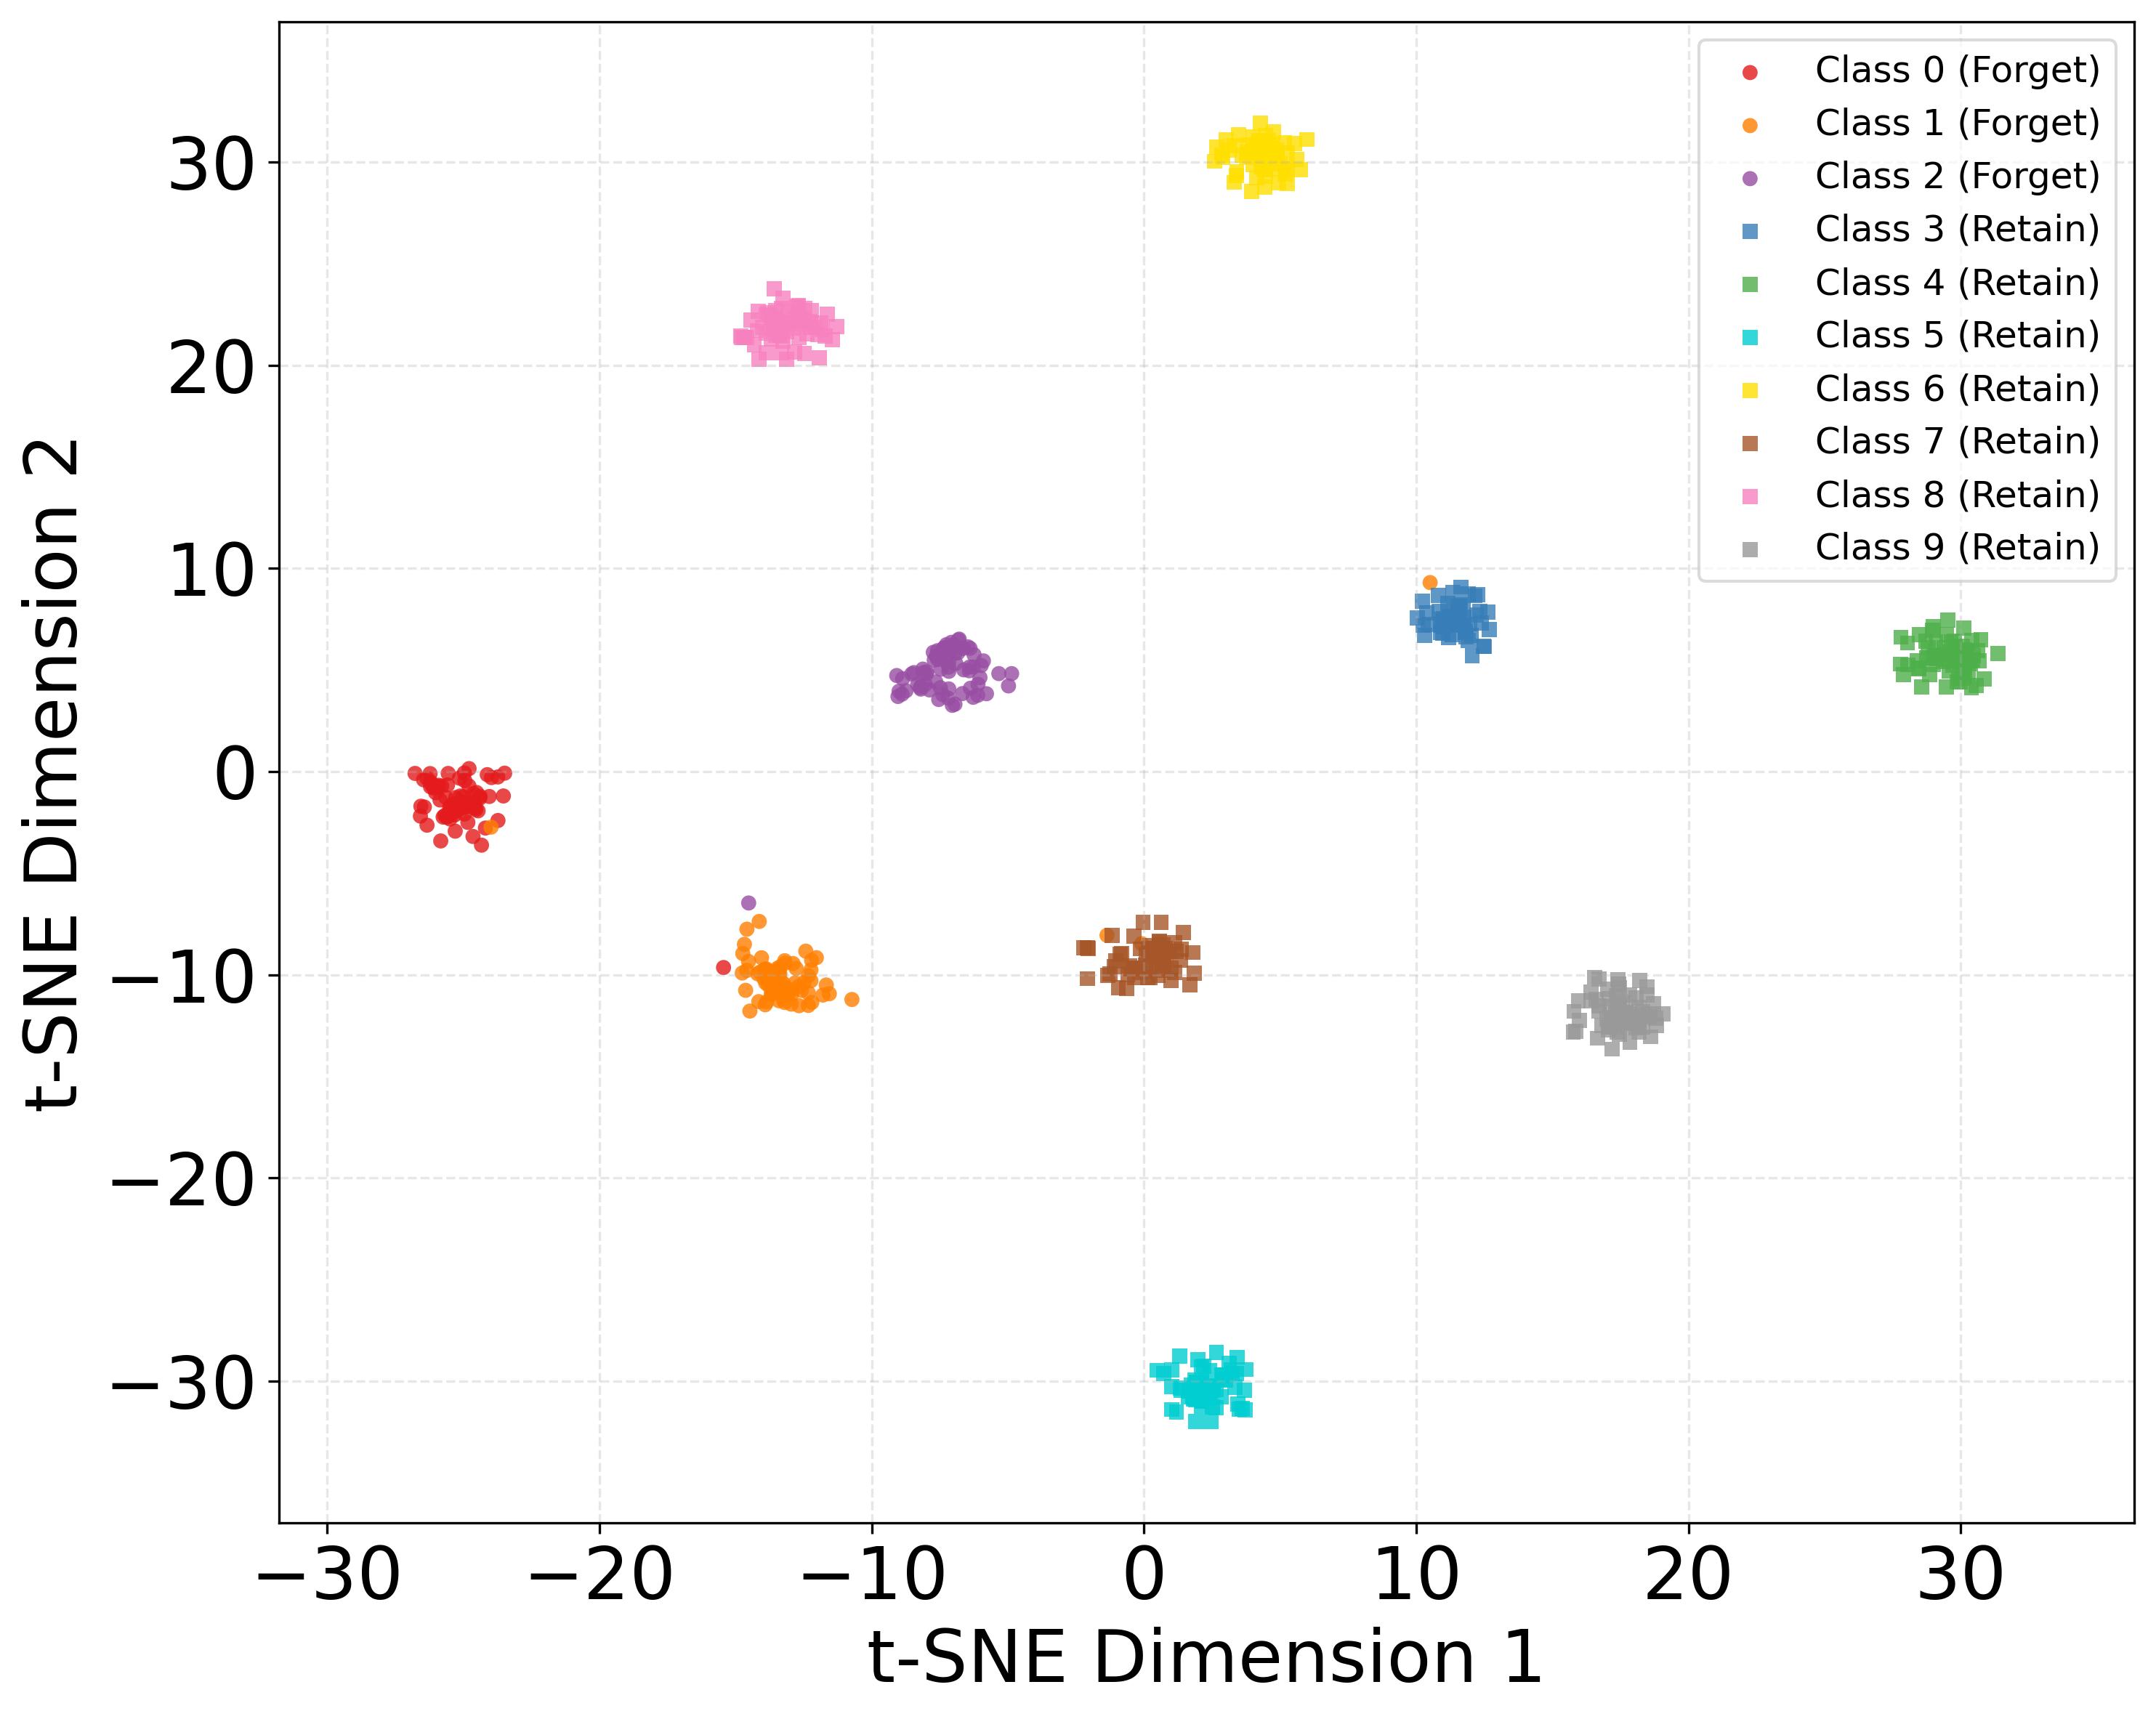
\includegraphics[width=0.45\linewidth]{tsne/base.png}
    \hfill
    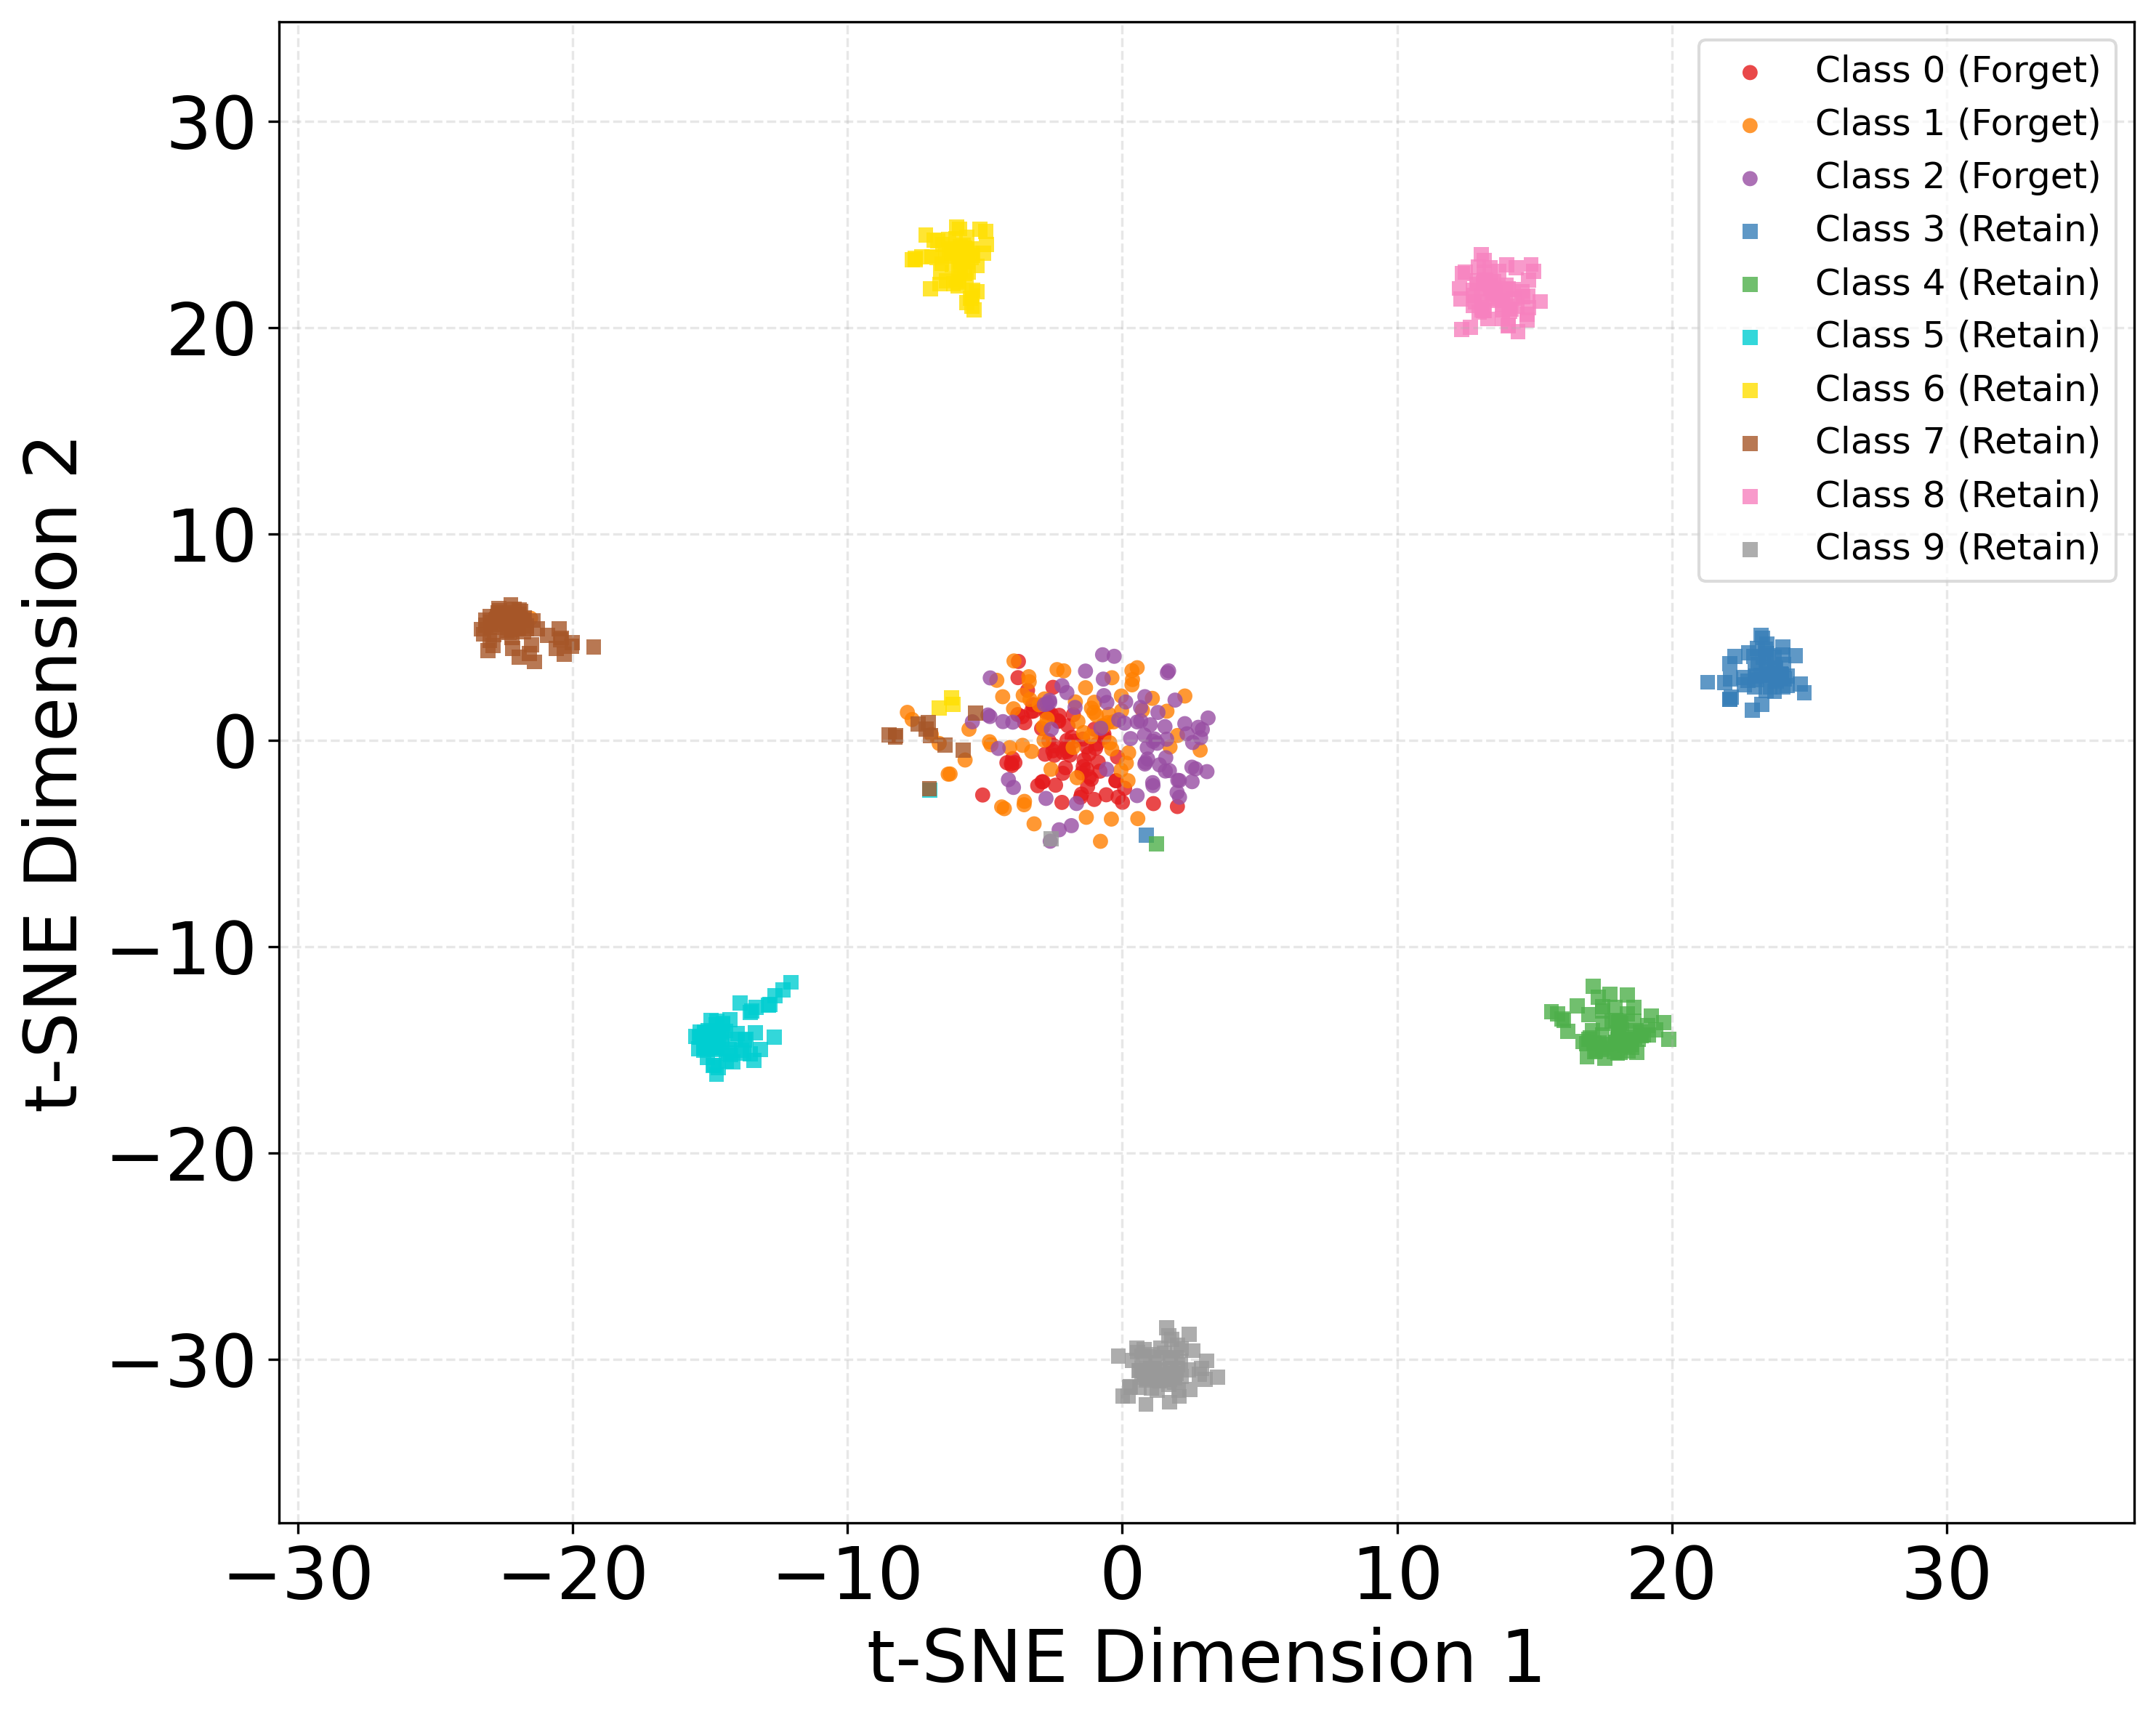
\includegraphics[width=0.45\linewidth]{tsne/GA.png}

    \vspace{0.3em}
    \makebox[0.45\linewidth]{\small (a) Initial}
    \hfill
    \makebox[0.45\linewidth]{\small (b) GS-LoRA}
    \vspace{1em}

    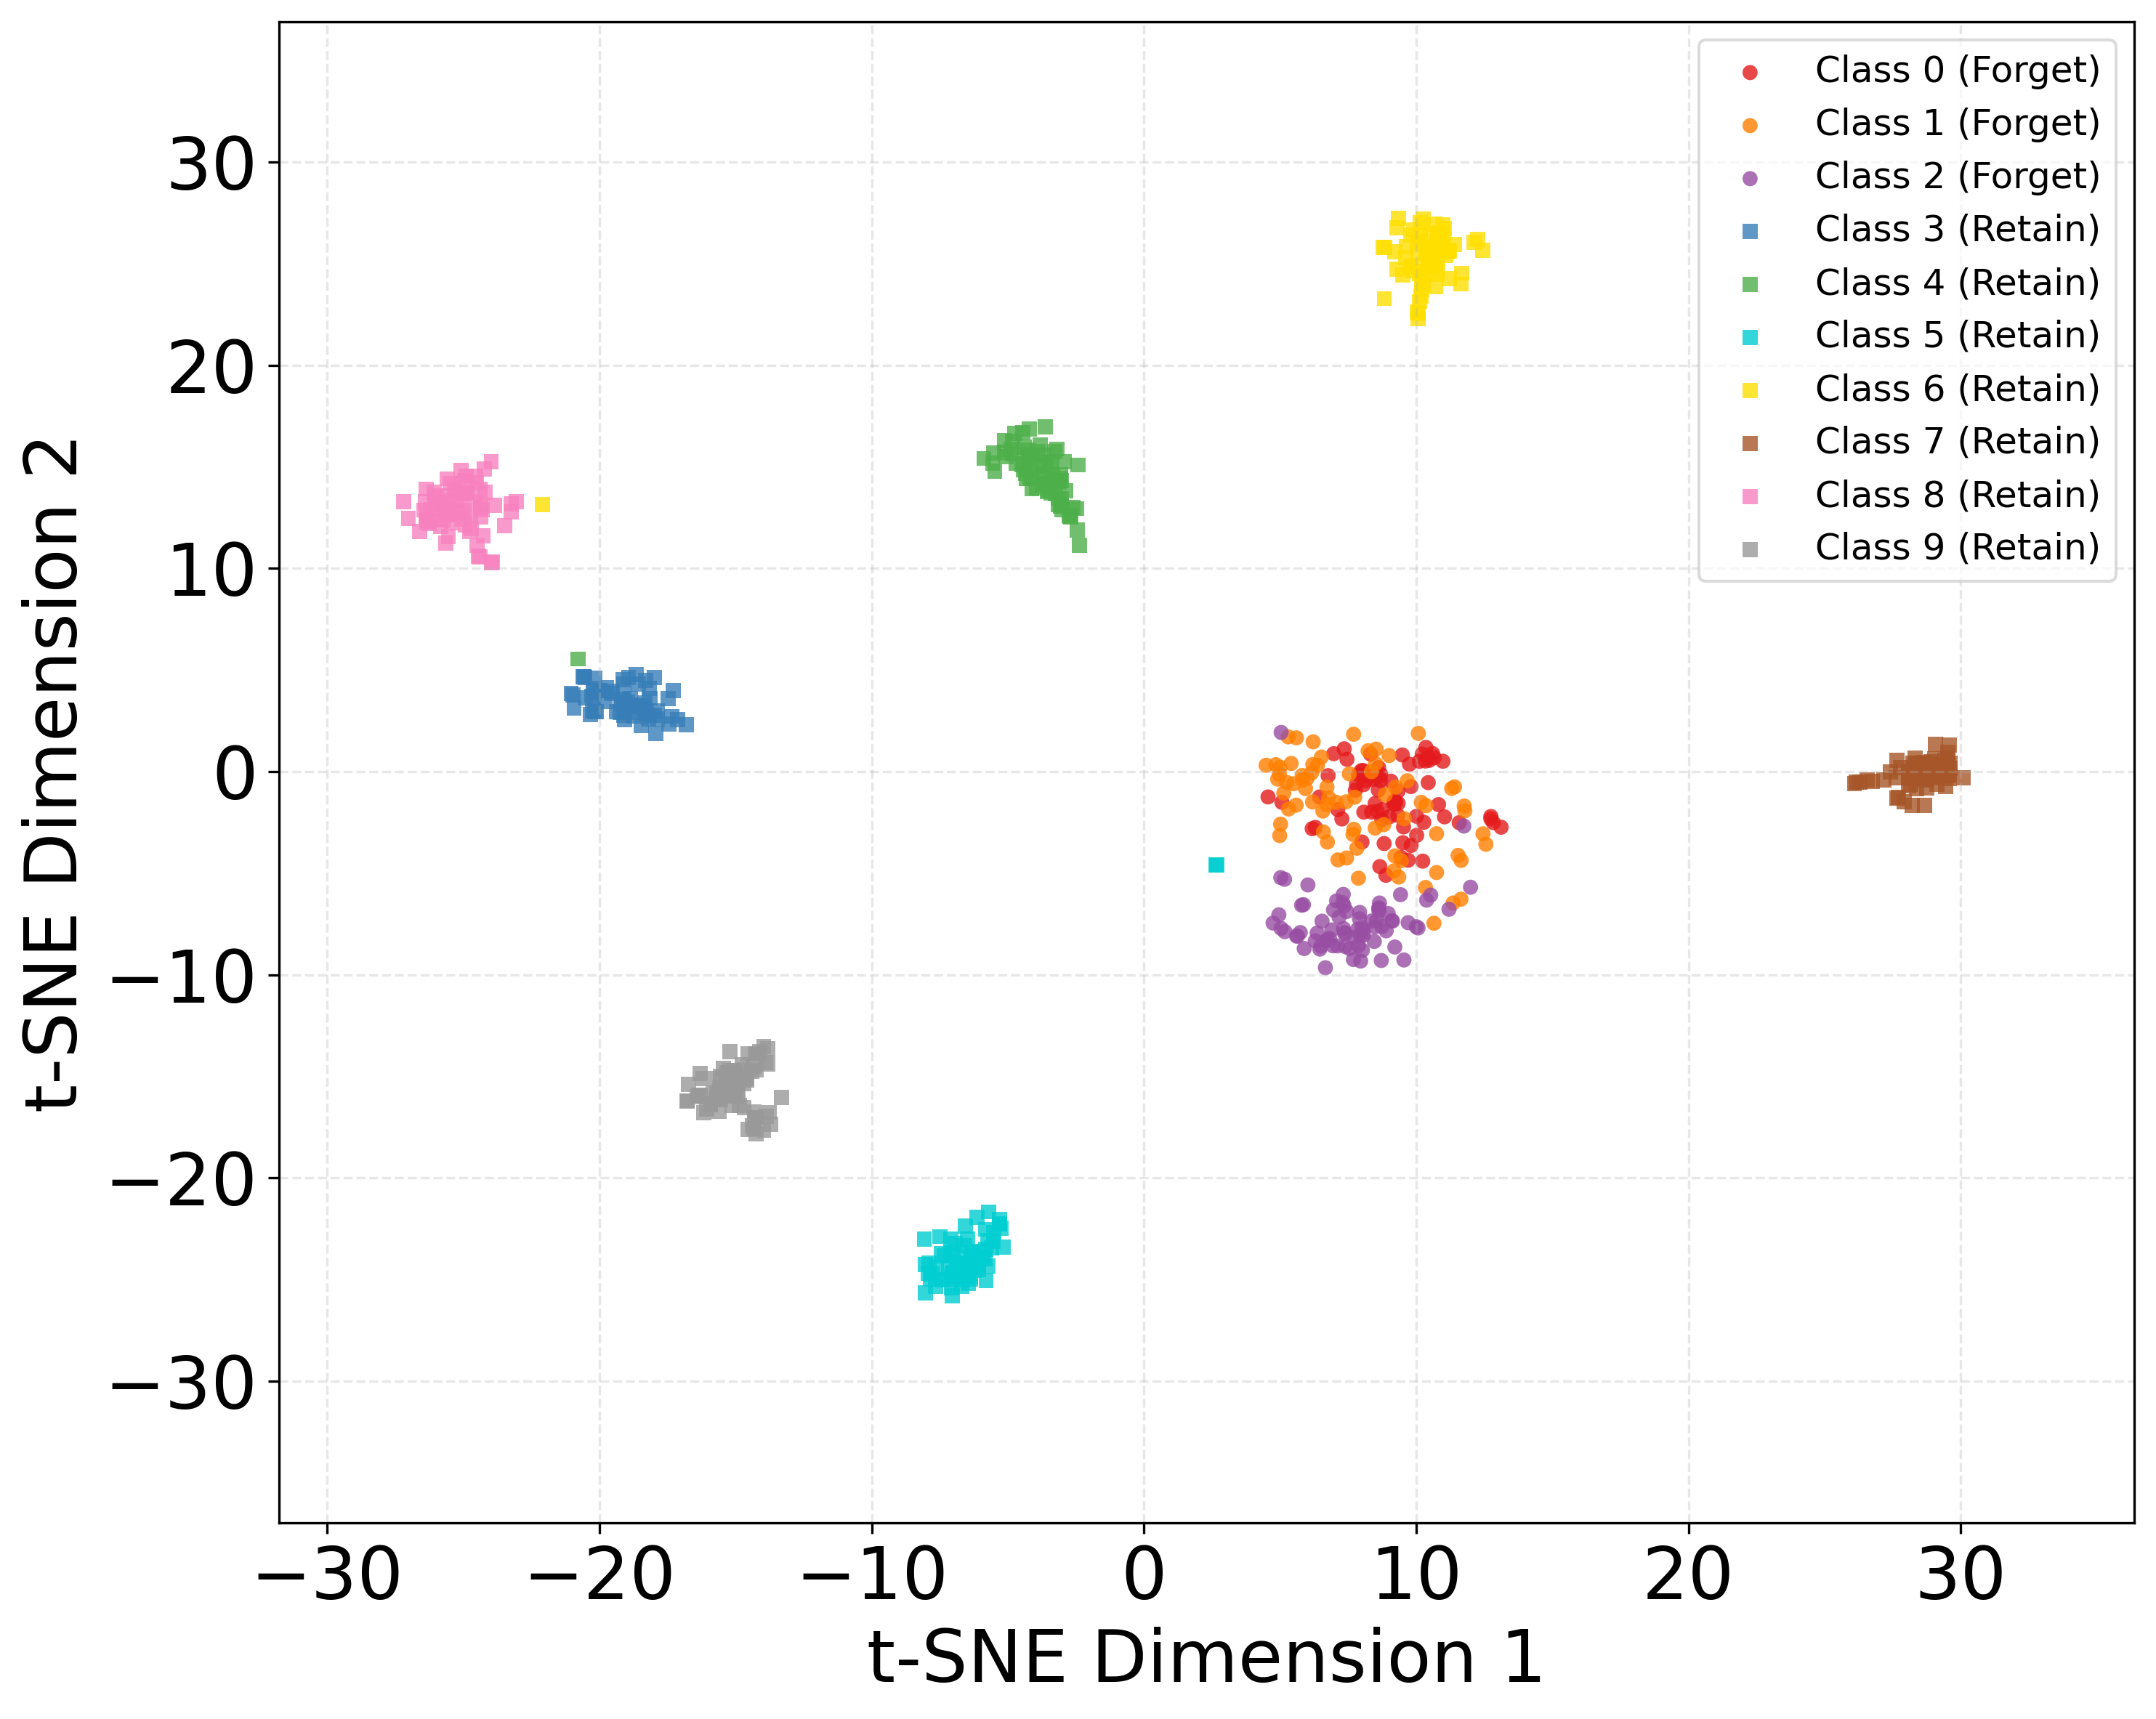
\includegraphics[width=0.45\linewidth]{tsne/shadow.png}
    \hfill
    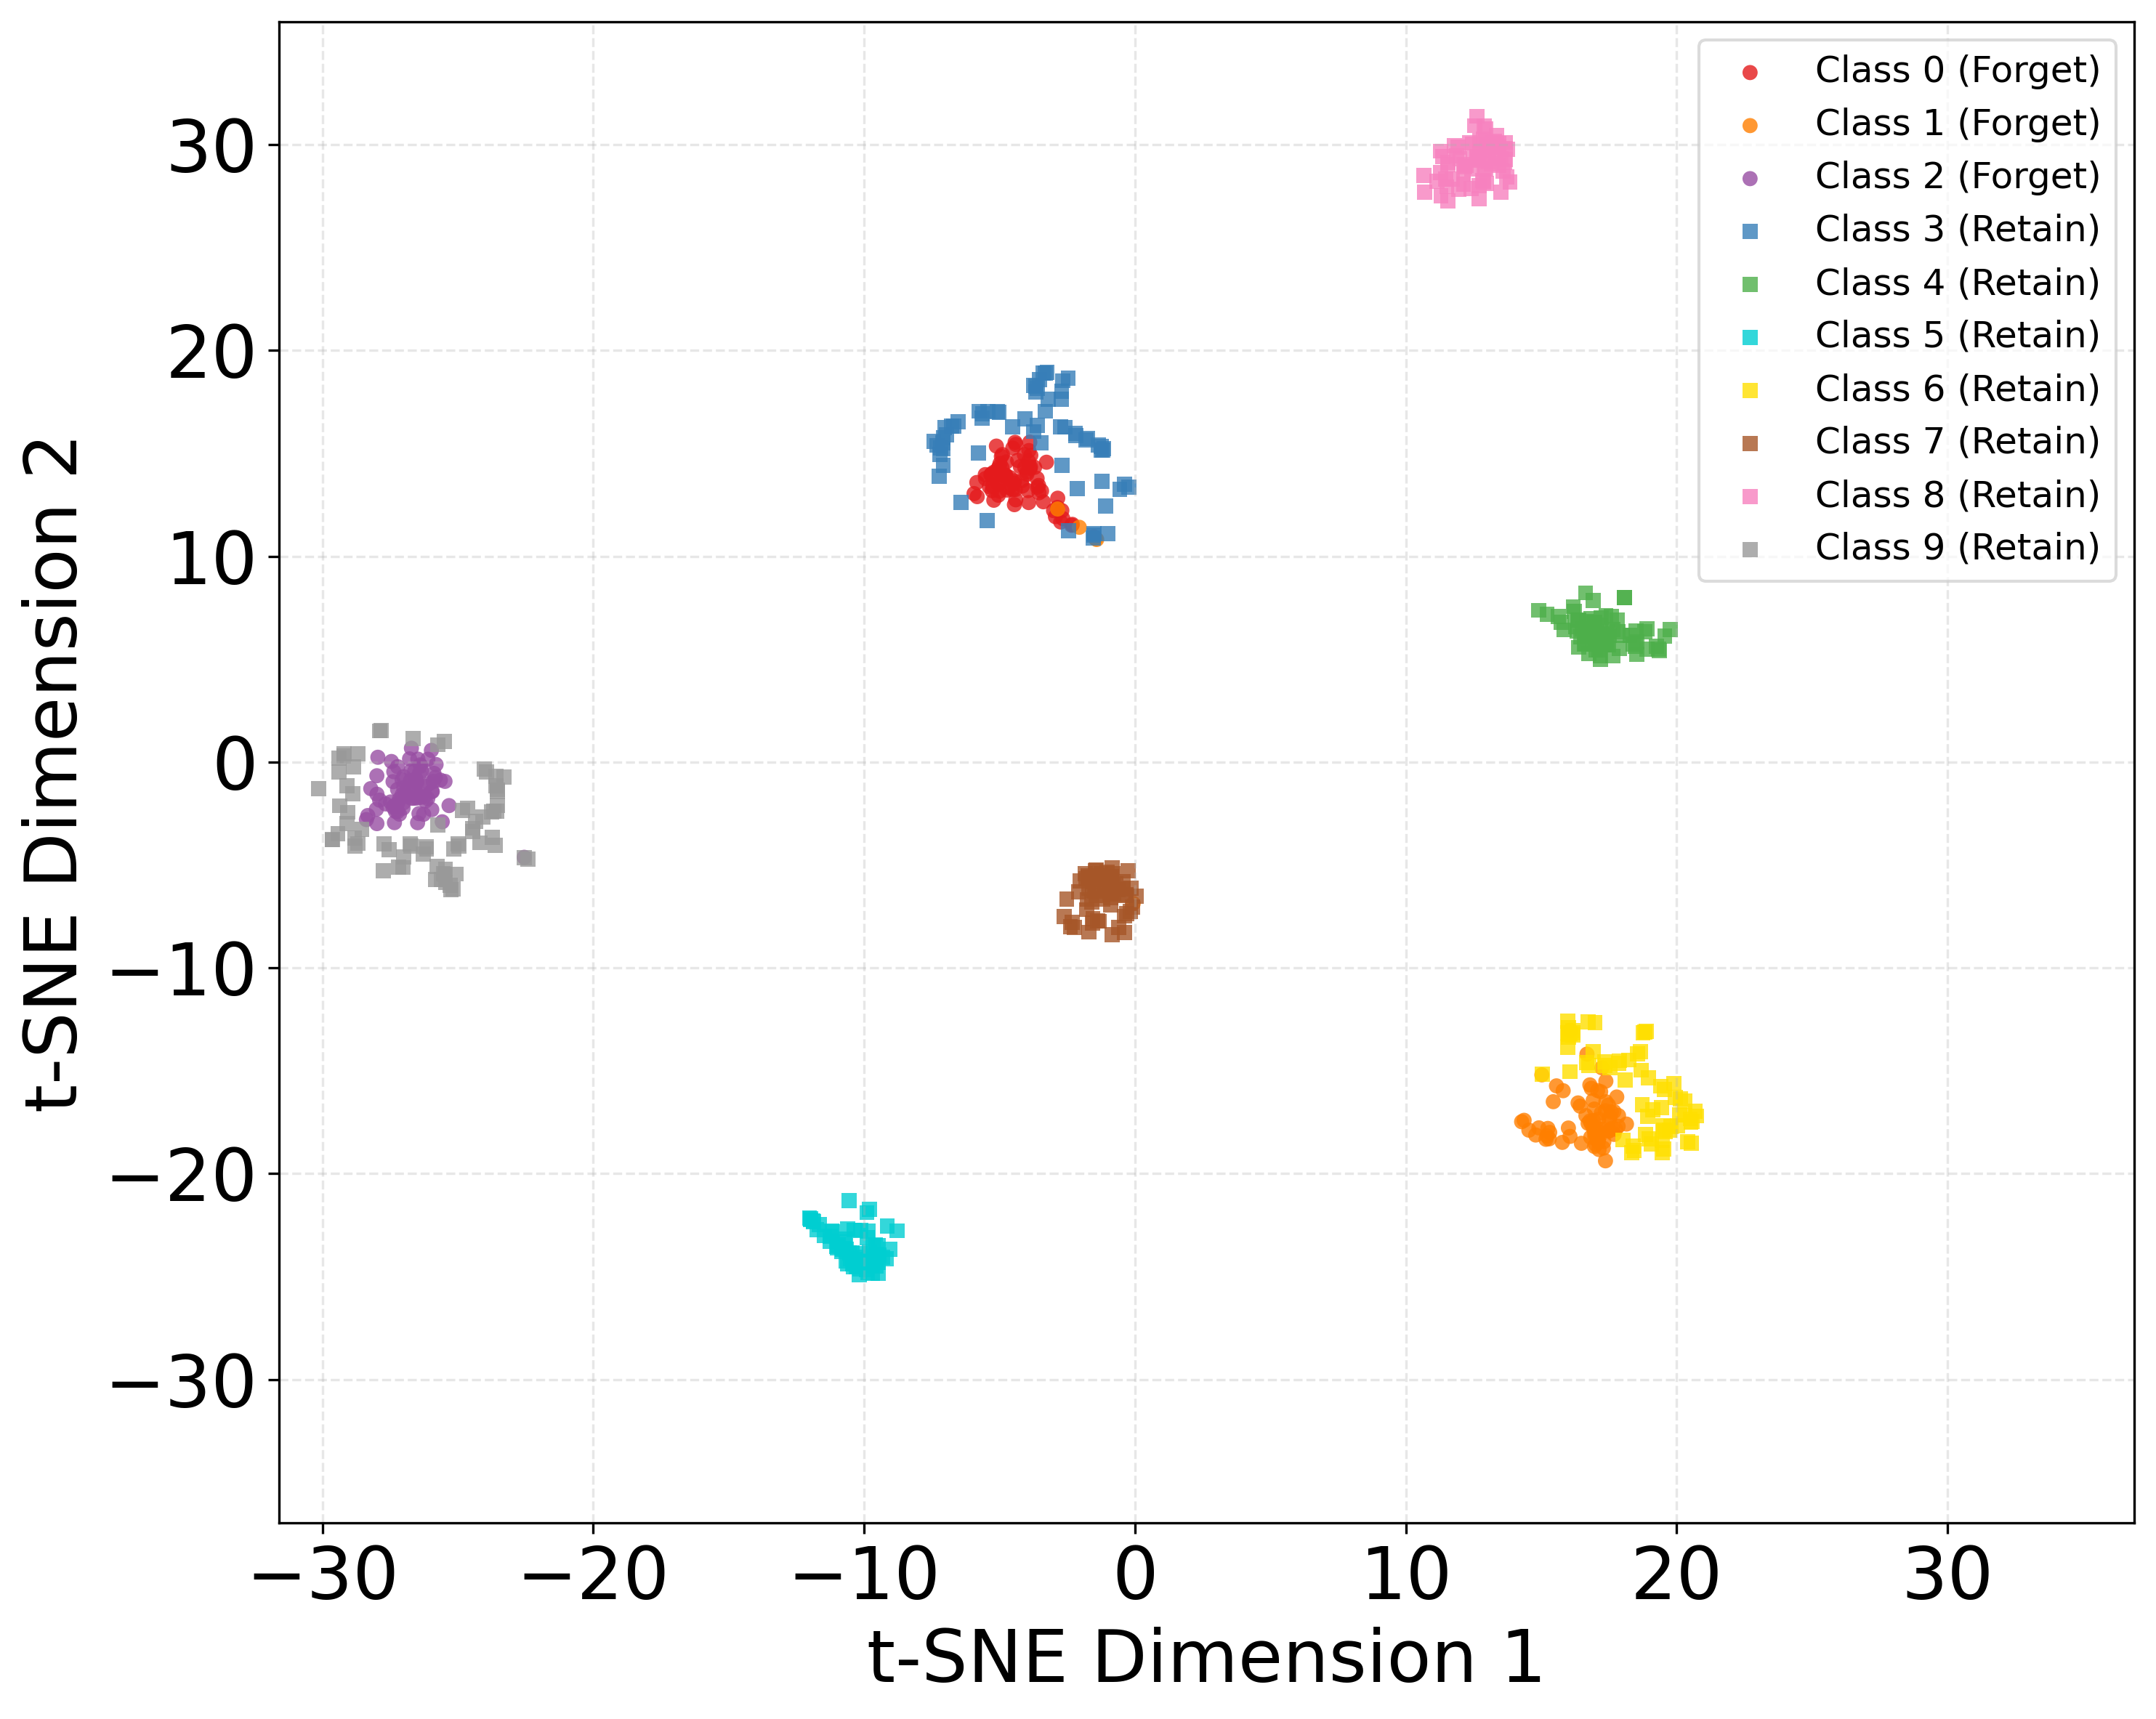
\includegraphics[width=0.45\linewidth]{tsne/cl.png}

    \vspace{0.3em}
    \makebox[0.45\linewidth]{\small (c) Boundary}
    \hfill
    \makebox[0.45\linewidth]{\small (d) CU (Ours)}

    \caption{t-SNE visualization. Baselines collapse to single point while proposed CU method distributes to nearest boundaries thus achieving faster convergence.}
    \label{fig:tsne_comparison}
\end{figure}

\subsection{Ablation Studies}
\vspace{0.2cm}
\noindent
We ablate three design choices on CIFAR-100: the replay buffer ratio $|D_\textbf{r}|$, the retain dominance constraint, and localized regularization. Table~\ref{tab:ablation_all} shows a 0.1 buffer ratio optimally balances retention and efficiency; the dominance constraint reduces $Acc_f$ from 9.97\% to 0.39\% by eliminating the long-tail convergence issue; and localized regularization reduces total $\ell_2$ norm from 39.05 to 10.09 with minimal retention loss, with Figure~\ref{fig:local_effect} showing the updates concentrate in specific blocks.

\begin{table}[!ht]
\centering
\small
\begin{tabular}{llccc}
\toprule
\textbf{Ablation} & \textbf{Setting} & $Acc_f{\downarrow}$ & $Acc_r{\uparrow}$ & \textbf{Extra} \\
\midrule
\multirow{4}{*}{Buffer Ratio $|D_r|$}
 & 1.0 (1$\times$)   & 1.33 & 74.39 & $H$=2.62 \\
 & 0.5 (2$\times$)   & 1.18 & 73.00 & $H$=2.32 \\
 & 0.3 (3.3$\times$) & 1.33 & 74.55 & $H$=2.61 \\
 & \cellcolor{orange!10}0.1 (10$\times$) & \cellcolor{orange!10}1.30 & \cellcolor{orange!10}74.52 & \cellcolor{orange!10}$H$=2.56 \\
\midrule
\multirow{2}{*}{Dominance Constraint}
 & Without & 9.97 & 78.12 & -- \\
 & \cellcolor{orange!10}With & \cellcolor{orange!10}0.39 & \cellcolor{orange!10}77.06 & \cellcolor{orange!10}-- \\
\midrule
\multirow{2}{*}{Localized Reg.}
 & Without & 0.00 & 77.24 & $\ell_2$=39.05 \\
 & \cellcolor{orange!10}With & \cellcolor{orange!10}0.00 & \cellcolor{orange!10}74.76 & \cellcolor{orange!10}$\ell_2$=10.09 \\
\bottomrule
\end{tabular}
\vspace{0.2cm}
\caption{Design ablations: replay buffer ratio, retain dominance constraint, and localized regularization on CIFAR-100. Highlighted rows are CU's default setting.}
\label{tab:ablation_all}
\end{table}

\begin{figure}[!ht]
    \centering
    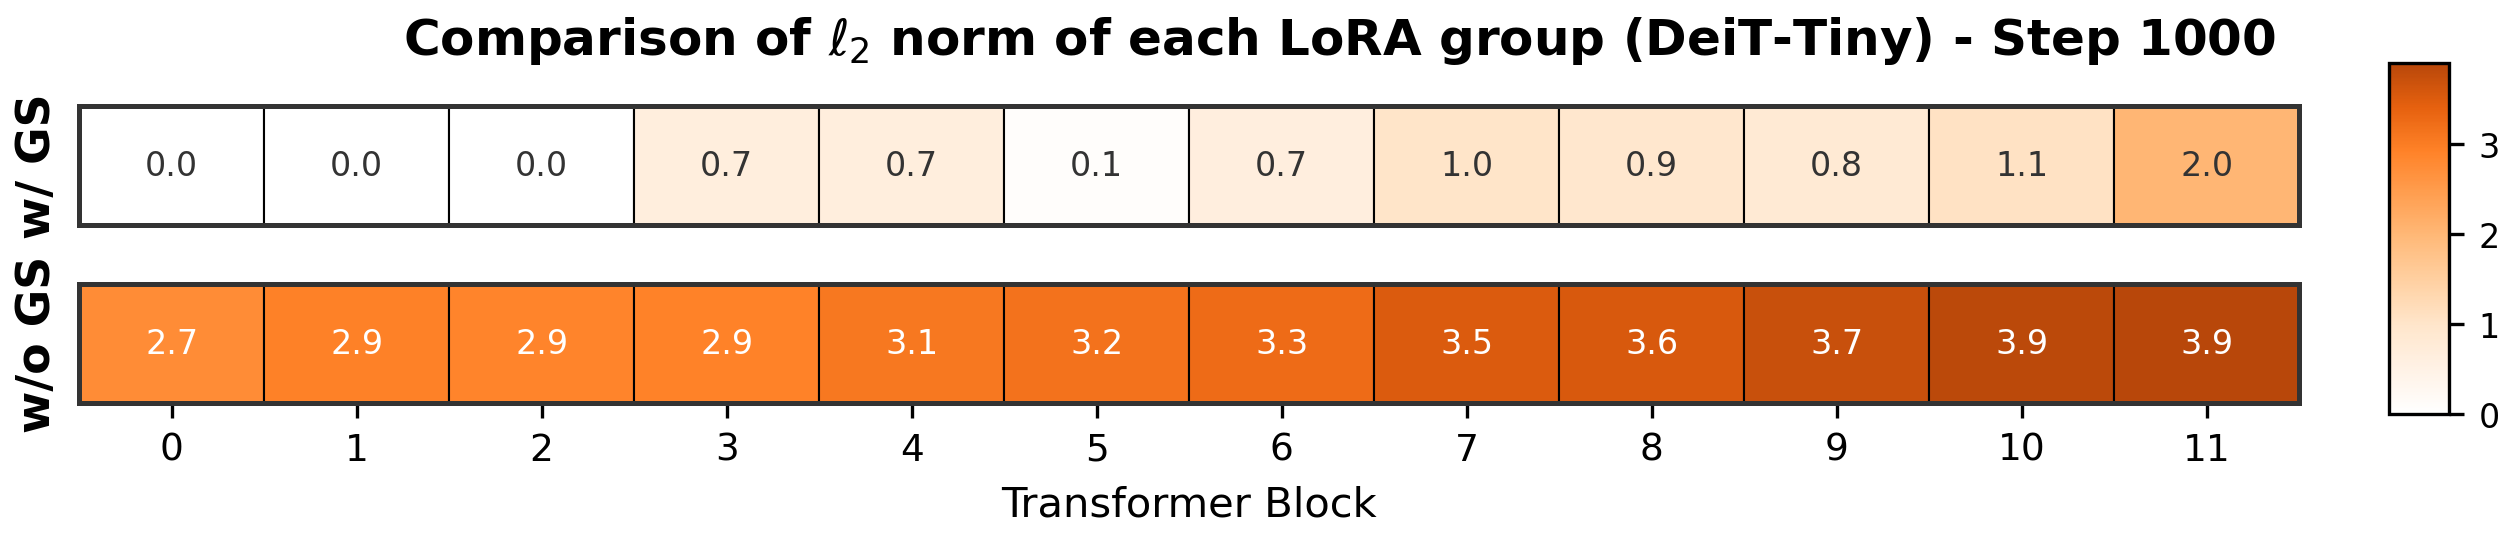
\includegraphics[width=1\linewidth]{images/GS.png}
    \caption{$\ell_2$ norm per block. Localized regularization concentrates updates in specific blocks.}
    \label{fig:local_effect}
\end{figure}

\subsection{Attack-Based Verification}
\label{sec:attack}
\vspace{0.2cm}
\noindent
\textcolor{red}{Table~\ref{tab:attack_verification}(a) reports FAR/EER of forget-class probes matched against the retain gallery on CASIA-Iris. CU tracks the Oracle closely (FAR@0.5 $3.83\%$ vs.\ $3.10\%$; EER $24.99\%$ vs.\ $21.69\%$), and both rise similarly over \textit{Before} unlearning ($1.64\%$), indicating that the small increase in open-set false accepts stems from removing the identities rather than from CU specifically.}

\textcolor{red}{Whether these residual accepts concentrate on one specific retained identity, a targeted per-identity vulnerability rather than a general accuracy shift, is a separate question. Beyond the $Acc_f$, KL, and confidence-based MIA already reported in Table~\ref{tab:all}, Table~\ref{tab:attack_verification}(b) reports six further attack-based tests on CASIA-Face100 after all forget identities are removed, each referenced against the \emph{Oracle} (retrain, information absent); values are placeholders pending final runs. The assigned-centroid match rate, each forget probe's match rate against its specifically \emph{assigned} nearest retain centroid, is no more frequent for CU than for Oracle, ruling out a concentrated, backdoor-like false-accept behavior between individual forget--retain identity pairs. The low linear-probe and slow relearning rates show forgetting is diffuse and not easily reversed, while label-only and adaptive MIA near chance and a low inversion match rate show that stronger, adaptive attacks fail as well. Results are empirical and attack-relative, not a formal guarantee, and directly support the retain-buffer necessity argument of Section~\ref{8.1}.}

\begin{table}[!ht]
\centering
\small
\setlength{\tabcolsep}{4pt}
\textcolor{red}{
\textbf{(a) FAR/EER on CASIA-Iris}\\[3pt]
\begin{tabular}{lcccc}
\toprule
Model & FAR@0.3 & FAR@0.4 & FAR@0.5 & EER \\
\midrule
Before & 11.38\% & 4.84\% & 1.64\% & 13.33\% \\
\rowcolor{orange!10}
CU & 17.97\% & 8.52\% & 3.83\% & 21.99\% \\
Oracle & 16.10\% & 7.79\% & 3.10\% & 21.69\% \\
\bottomrule
\end{tabular}
\vspace{0.3cm}
\textbf{(b) Attack-based confound tests on CASIA-Face100}\\[3pt]
\scriptsize
\begin{tabular}{lcc}
\toprule
\textbf{Test} & \textbf{CU} & \textbf{Oracle} \\
\midrule
Assigned-centroid match $\downarrow$ & \textbf{3.91} & 3.74 \\
\midrule
Linear probe (frozen emb.) $\downarrow$ & \textbf{6.28} & 4.65 \\
5-shot relearn $Acc_f$ $\downarrow$ & \textbf{5.47} & 6.12 \\
\midrule
MIA, label-only~\cite{choquette2021label} $\approx\!0.5$ & \textbf{0.53} & 0.51 \\
MIA, adaptive $\approx\!0.5$ & \textbf{0.54} & 0.50 \\
Model inversion match $\downarrow$ & \textbf{3.62} & 3.98 \\
\bottomrule
\end{tabular}}
\vspace{0.15cm}
\caption{\textcolor{red}{Attack-based verification. (a) FAR/EER of forget-class probes against the retain gallery on CASIA-Iris. (b) Six further attack-based tests on CASIA-Face100, complementing the $Acc_f$, KL, and MIA results of Table~\ref{tab:all}. Values in (b) are placeholders pending final runs.}}
\label{tab:attack_verification}
\end{table}
